\documentclass[a4paper,12pt]{article}

\usepackage[margin=2cm]{geometry}
\usepackage{tikz}
\usepackage[T1]{fontenc}
\usepackage{lmodern}
\usepackage{float}
\usepackage{caption}

\usetikzlibrary{shapes.geometric, arrows.meta, positioning, fit, calc}

% ==================== STYLES ====================
\tikzset{
    startstop/.style={circle, fill=black, minimum size=8mm, inner sep=0pt},
    activity/.style={rectangle, draw, minimum width=3cm, minimum height=0.8cm, align=center, font=\small},
    decision/.style={diamond, draw, minimum width=1.5cm, minimum height=1cm, align=center, font=\small, aspect=2},
    arrow/.style={-{Stealth[length=2.5mm]}, thick},
    usecase/.style={ellipse, draw, minimum width=3cm, minimum height=1cm, align=center, font=\small},
    sysbox/.style={rectangle, draw, inner sep=10pt},
    entityheader/.style={rectangle, draw, fill=black!8, minimum width=4.5cm,
                         minimum height=0.7cm, align=center, font=\small\bfseries},
    entityrow/.style={rectangle, draw, minimum width=4.5cm, minimum height=0.5cm,
                      align=left, font=\scriptsize, inner xsep=4pt},
    process/.style={circle, draw, minimum size=1.8cm, align=center, font=\small},
    datastore/.style={rectangle, draw, minimum width=2.8cm, minimum height=0.65cm,
                      align=center, font=\scriptsize},
    external/.style={rectangle, draw, minimum width=2.4cm, minimum height=0.9cm,
                     align=center, font=\small},
    dataflow/.style={-{Stealth[length=2.5mm]}, thick},
    biflow/.style={{Stealth[length=2.5mm]}-{Stealth[length=2.5mm]}, thick},
    lbl/.style={font=\scriptsize, fill=white, inner sep=1pt},
}

\newcommand{\stickfigure}[3]{%
    \draw (#1,#2+0.4) circle (0.15);
    \draw (#1,#2+0.25) -- (#1,#2-0.05);
    \draw (#1-0.2,#2+0.15) -- (#1+0.2,#2+0.15);
    \draw (#1,#2-0.05) -- (#1-0.15,#2-0.35);
    \draw (#1,#2-0.05) -- (#1+0.15,#2-0.35);
    \node[font=\small, below] at (#1,#2-0.4) {#3};
}

\begin{document}

% ── TITLE ────────────────────────────────────────────────────────────
\begin{center}
    {\Huge\bfseries FitAxis}\\[8pt]
    {\Large Software Design Diagrams}\\[16pt]
    \rule{0.6\textwidth}{0.5pt}\\[12pt]
    {\normalsize Activity Diagram \quad$\bullet$\quad Use Case Diagram \quad$\bullet$\quad
     ER Diagram \quad$\bullet$\quad DFD Level~0 \quad$\bullet$\quad DFD Level~1}\\[12pt]
    \rule{0.6\textwidth}{0.5pt}\\[8pt]
    {\small Fitness Tracking Application --- Flutter \& Firebase}
\end{center}
\clearpage

% =====================================================================
% 1. ACTIVITY DIAGRAM
% =====================================================================
\subsection*{Activity Diagram}
The activity diagram illustrates the workflow of the FitAxis system from app launch through user authentication and feature usage.

\begin{figure}[H]
\centering
\resizebox{0.85\textwidth}{!}{%
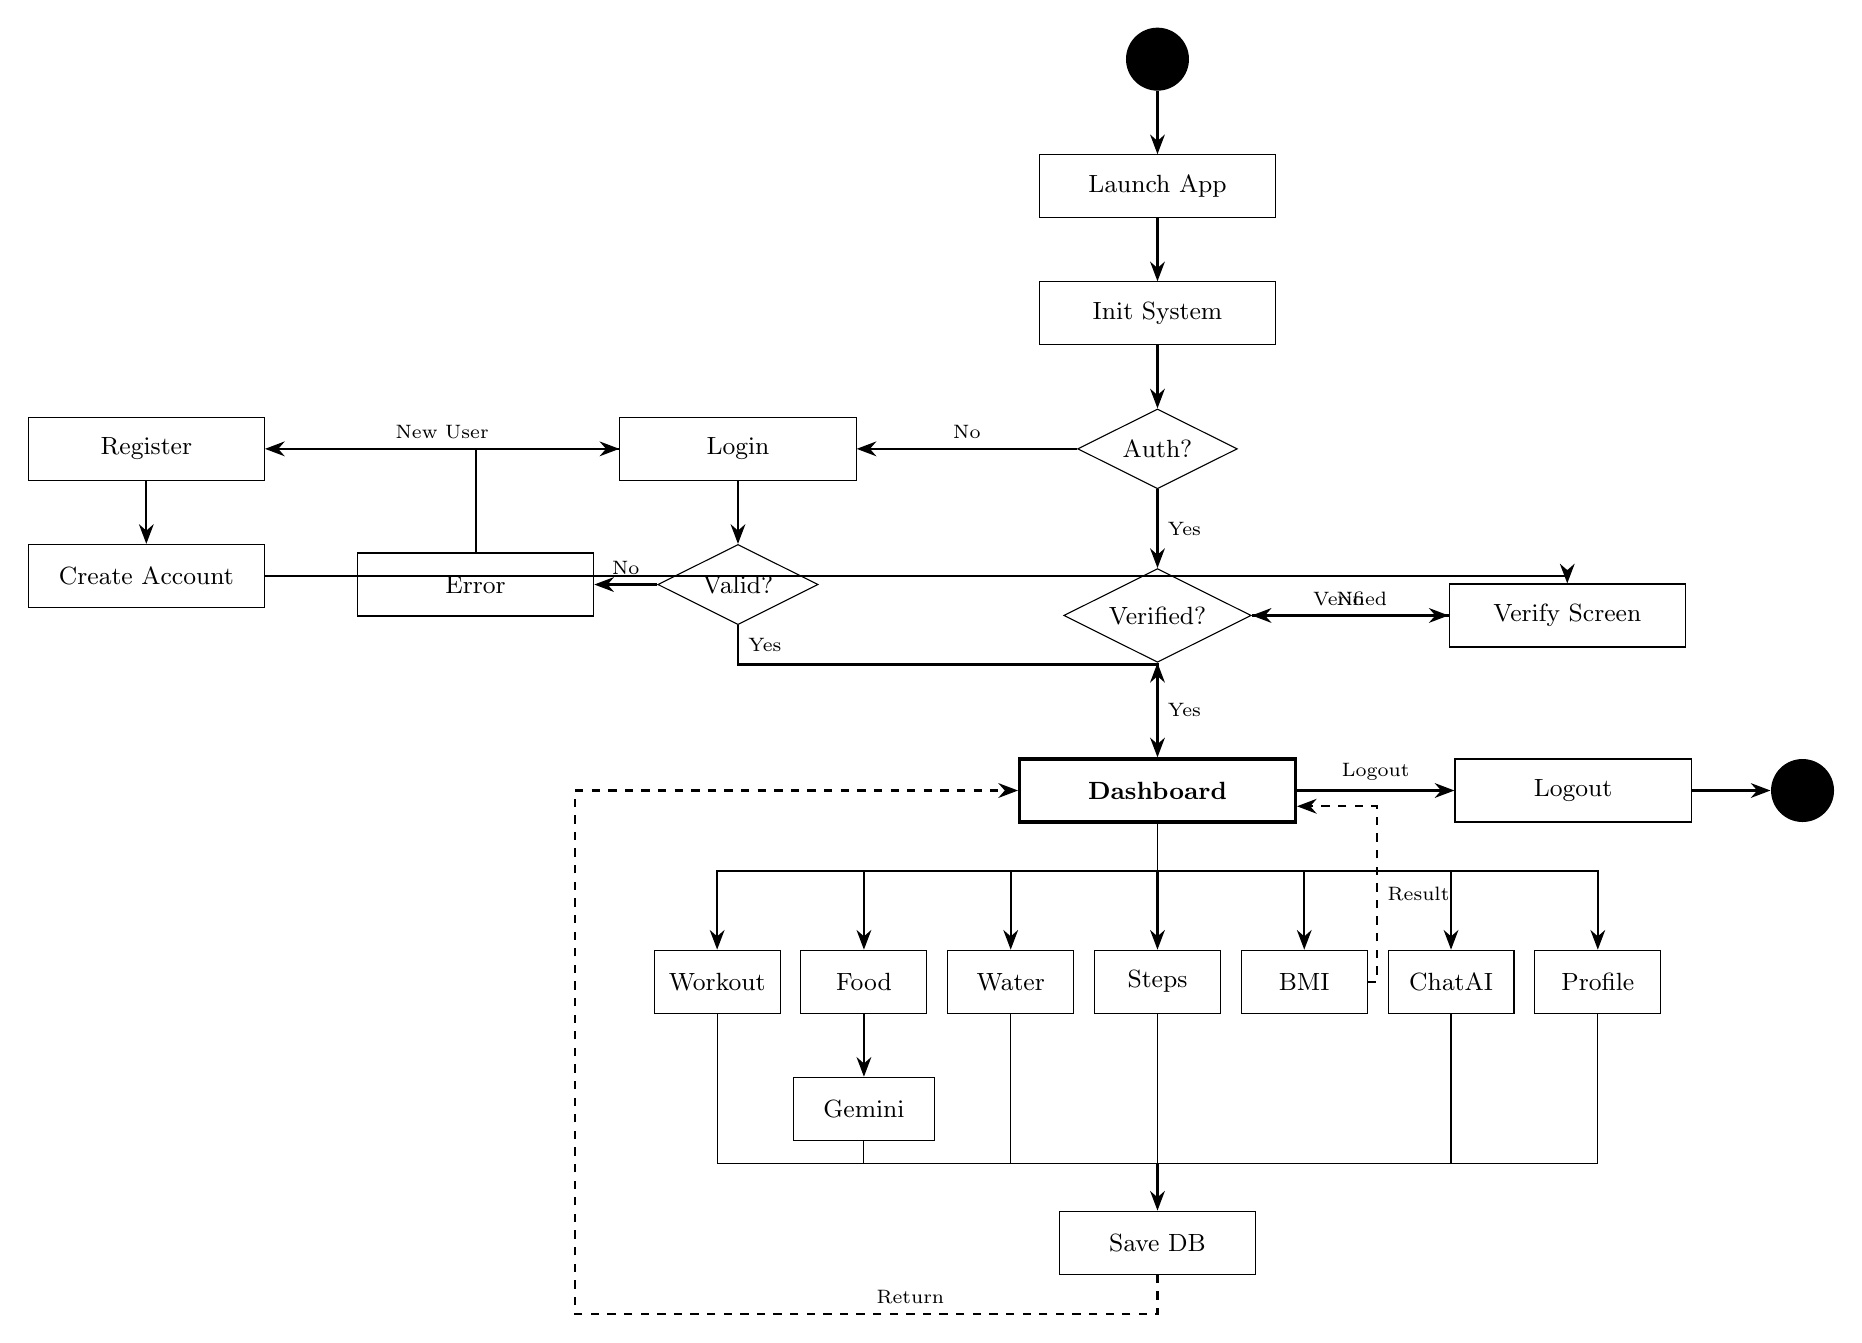
\begin{tikzpicture}[node distance=1cm and 1.5cm]

    \node[startstop] (start) {};

    \node[activity, below=0.8cm of start] (launch) {Launch App};
    \node[activity, below=0.8cm of launch] (init) {Init System};
    \node[decision, below=0.8cm of init] (authCheck) {Auth?};

    \node[activity, left=2.8cm of authCheck] (login) {Login};
    \node[decision, below=0.8cm of login] (validCreds) {Valid?};
    \node[activity, left=0.8cm of validCreds] (error) {Error};

    \node[activity, left=4.5cm of login] (register) {Register};
    \node[activity, below=0.8cm of register] (createAcc) {Create Account};

    \node[decision, below=1cm of authCheck] (emailCheck) {Verified?};
    \node[activity, right=2.5cm of emailCheck] (verifyScreen) {Verify Screen};

    \node[activity, below=1.2cm of emailCheck, minimum width=3.5cm, line width=1.2pt]
        (dashboard) {\textbf{Dashboard}};

    % 7 core actions horizontally nested under dashboard to prevent width overload
    \node[activity, minimum width=1.6cm, below=1.6cm of dashboard] (steps) {Steps};
    \node[activity, minimum width=1.6cm, left=0.25cm of steps] (water) {Water};
    \node[activity, minimum width=1.6cm, left=0.25cm of water] (food) {Food};
    \node[activity, minimum width=1.6cm, left=0.25cm of food] (workout) {Workout};

    \node[activity, minimum width=1.6cm, right=0.25cm of steps] (bmi) {BMI};
    \node[activity, minimum width=1.6cm, right=0.25cm of bmi] (chatbot) {ChatAI};
    \node[activity, minimum width=1.6cm, right=0.25cm of chatbot] (profile) {Profile};

    \node[activity, minimum width=1.8cm, below=0.8cm of food] (gemini) {Gemini};
    \node[activity, minimum width=2.5cm, below=2.5cm of steps] (save) {Save DB};

    \node[activity, right=2cm of dashboard] (logout) {Logout};
    \node[startstop, right=1cm of logout] (endNode) {};

    \draw[arrow] (start) -- (launch);
    \draw[arrow] (launch) -- (init);
    \draw[arrow] (init) -- (authCheck);
    
    \draw[arrow] (authCheck) -- node[above, font=\scriptsize] {No} (login);
    \draw[arrow] (authCheck) -- node[right, font=\scriptsize] {Yes} (emailCheck);
    
    \draw[arrow] (login) -- (validCreds);
    \draw[arrow] (validCreds) -- node[above, font=\scriptsize] {No} (error);
    \draw[arrow] (error) |- (login);
    
    \draw[arrow] (validCreds) -- node[right, font=\scriptsize] {Yes}
        ([yshift=-0.5cm]validCreds.south) -| (emailCheck);
        
    \draw[arrow] (login) -- node[above, font=\scriptsize] {New User} (register);
    \draw[arrow] (register) -- (createAcc);
    \draw[arrow] (createAcc) -| (verifyScreen);
    
    \draw[arrow] (emailCheck) -- node[above, font=\scriptsize] {No} (verifyScreen);
    \draw[arrow] (verifyScreen) -- node[above, font=\scriptsize] {Verified} (emailCheck);
    \draw[arrow] (emailCheck) -- node[right, font=\scriptsize] {Yes} (dashboard);

    \draw[arrow] (dashboard) -- node[above, font=\scriptsize] {Logout} (logout);
    \draw[arrow] (logout) -- (endNode);

    % Main spine connecting dashboard to the 7 modules vertically down and spanning horizontal
    \coordinate (dash_out) at ([yshift=-0.6cm]dashboard.south);
    \draw[-] (dashboard.south) -- (dash_out);
    \draw[arrow] (dash_out) -| (workout.north);
    \draw[arrow] (dash_out) -| (food.north);
    \draw[arrow] (dash_out) -| (water.north);
    \draw[arrow] (dash_out) -| (steps.north);
    \draw[arrow] (dash_out) -| (bmi.north);
    \draw[arrow] (dash_out) -| (chatbot.north);
    \draw[arrow] (dash_out) -| (profile.north);

    % Connecting modules properly down to Save DB
    \coordinate (save_in) at ([yshift=0.6cm]save.north);
    \draw[-] (workout.south) |- (save_in);
    \draw[-] (water.south) |- (save_in);
    \draw[-] (steps.south) |- (save_in);
    \draw[-] (chatbot.south) |- (save_in);
    \draw[-] (profile.south) |- (save_in);
    
    \draw[arrow] (food.south) -- (gemini.north);
    \draw[-] (gemini.south) |- (save_in);
    \draw[arrow] (save_in) -- (save.north);

    % Flow returns using safe bounds outer bounds
    \draw[arrow, dashed] (save.south) 
        -- ([yshift=-0.5cm]save.south) 
        -| node[near start, above right, font=\scriptsize] {Return} ([xshift=-1cm]workout.west) 
        |- (dashboard.west);
        
    \draw[arrow, dashed] (bmi.east) 
        -- ++(0.12,0) 
        |- node[near start, right, font=\scriptsize] {Result} ([yshift=-0.2cm]dashboard.east);

\end{tikzpicture}
}%
\caption{Activity Diagram --- FitAxis User Flow}
\end{figure}
\clearpage

% =====================================================================
% 2. USE CASE DIAGRAM
% =====================================================================
\subsection*{Use Case Diagram}

\begin{figure}[H]
\centering
\resizebox{0.9\textwidth}{!}{%
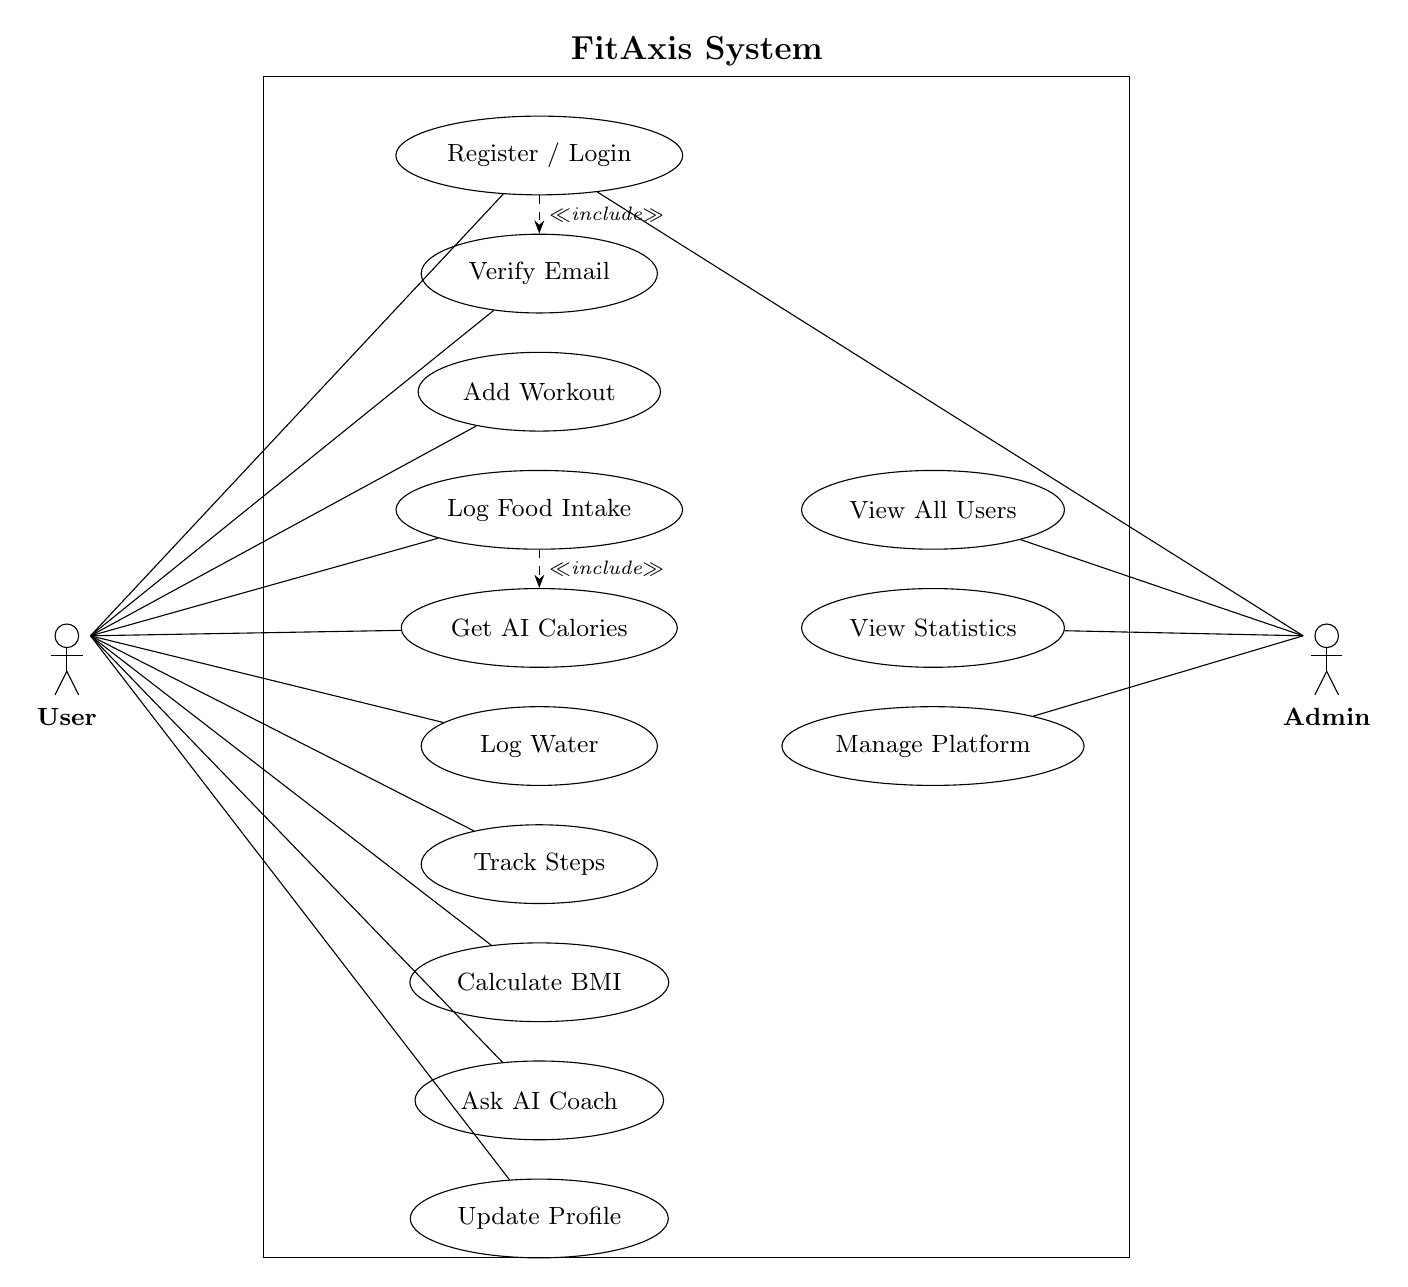
\begin{tikzpicture}

    % System boundary
    \node[sysbox, minimum width=11cm, minimum height=15cm,
          label={[font=\large\bfseries]above:FitAxis System}] (sys) {};

    % Actors
    \stickfigure{-8}{0}{\textbf{User}}
    \stickfigure{8}{0}{\textbf{Admin}}

    % User use cases (left column inside box)
    \node[usecase] at (-2, 6.5) (uc1)  {Register / Login};
    \node[usecase] at (-2, 5.0) (uc2)  {Verify Email};
    \node[usecase] at (-2, 3.5) (uc3)  {Add Workout};
    \node[usecase] at (-2, 2.0) (uc4)  {Log Food Intake};
    \node[usecase] at (-2, 0.5) (uc5)  {Get AI Calories};
    \node[usecase] at (-2,-1.0) (uc6)  {Log Water};
    \node[usecase] at (-2,-2.5) (uc7)  {Track Steps};
    \node[usecase] at (-2,-4.0) (uc8)  {Calculate BMI};
    \node[usecase] at (-2,-5.5) (uc9)  {Ask AI Coach};
    \node[usecase] at (-2,-7.0) (uc10) {Update Profile};

    % Admin use cases (right column inside box)
    \node[usecase] at (3, 2.0) (uc11) {View All Users};
    \node[usecase] at (3, 0.5) (uc12) {View Statistics};
    \node[usecase] at (3,-1.0) (uc13) {Manage Platform};

    % User connections
    \foreach \uc in {uc1,uc2,uc3,uc4,uc5,uc6,uc7,uc8,uc9,uc10}
        \draw (-7.7, 0.4) -- (\uc);

    % Admin connections
    \foreach \uc in {uc1,uc11,uc12,uc13}
        \draw (7.7, 0.4) -- (\uc);

    % Include / Extend
    \draw[dashed, -{Stealth}] (uc1) --
        node[right, font=\scriptsize\itshape] {$\ll$include$\gg$} (uc2);
    \draw[dashed, -{Stealth}] (uc4) --
        node[right, font=\scriptsize\itshape] {$\ll$include$\gg$} (uc5);

\end{tikzpicture}
}%
\caption{Use Case Diagram --- FitAxis System}
\end{figure}
\clearpage

% =====================================================================
% 3. ER DIAGRAM
% =====================================================================
\subsection*{ER Diagram}

\begin{figure}[H]
\centering
\resizebox{\textwidth}{!}{%
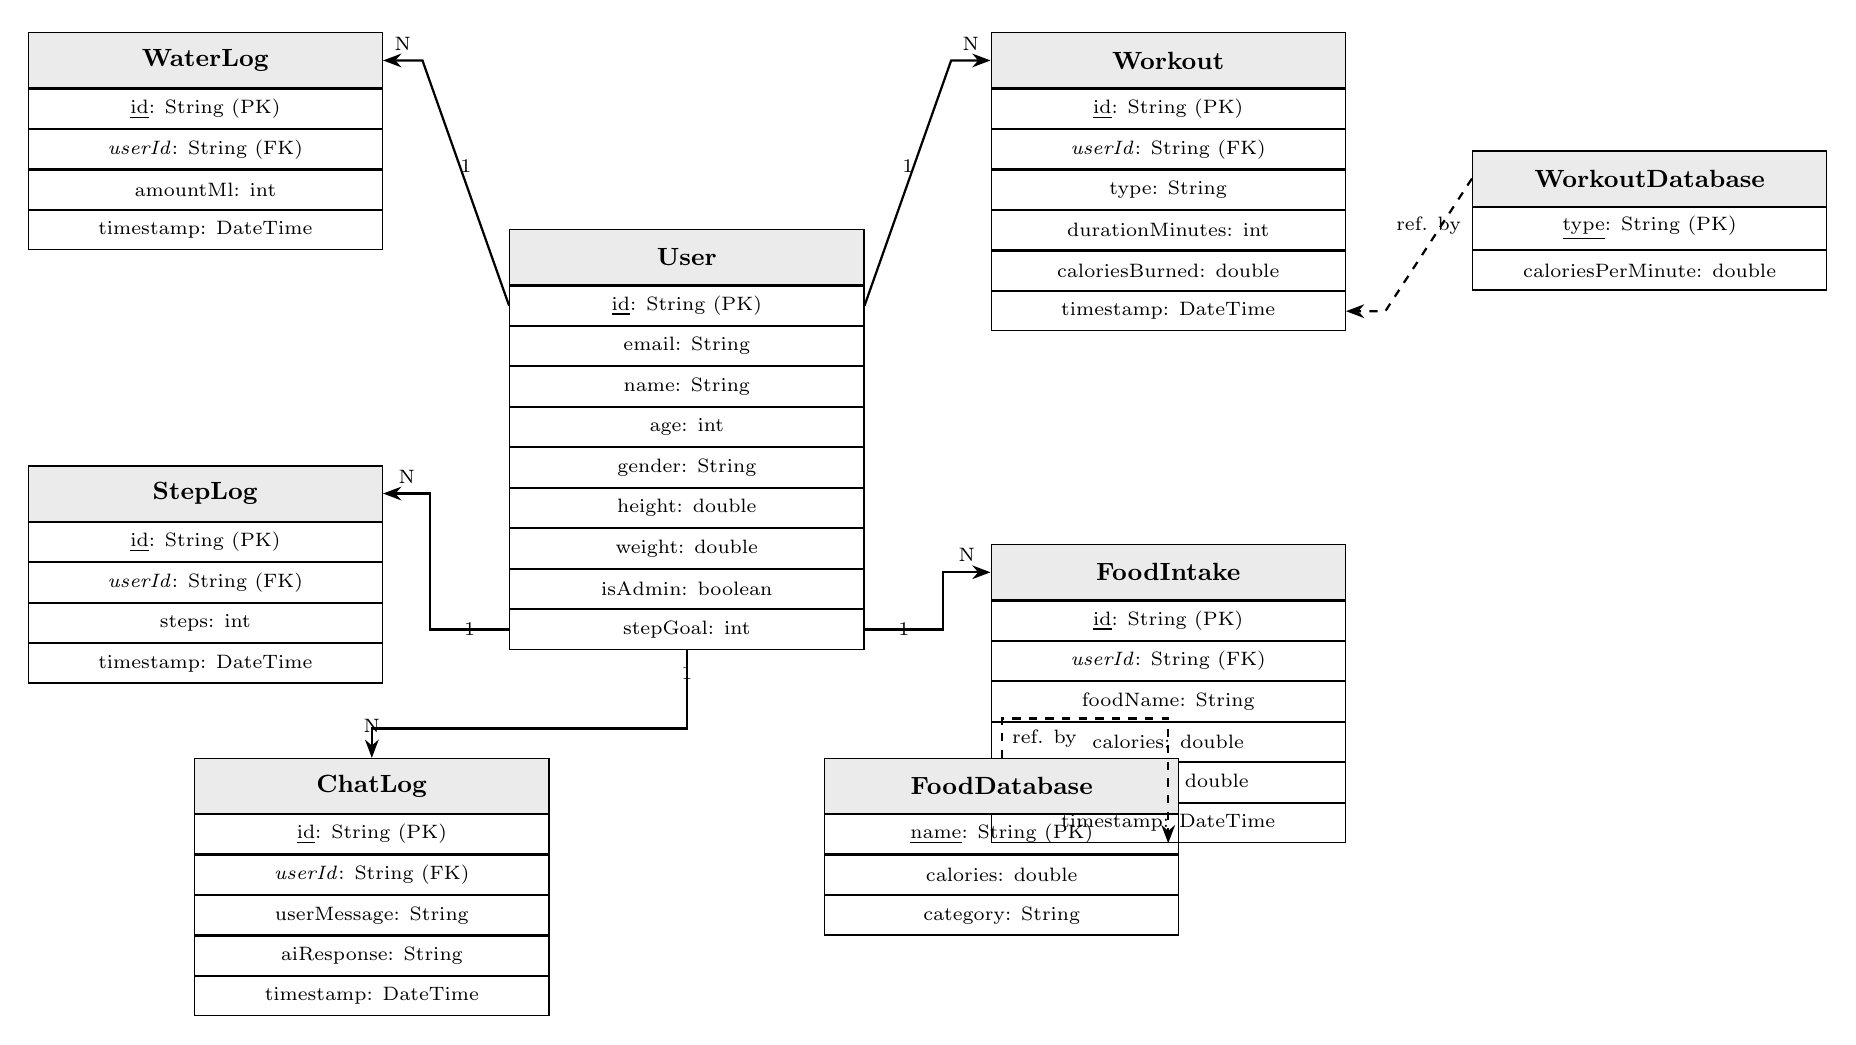
\begin{tikzpicture}[node distance=0.5cm and 3cm]

    % ── USER ──
    \node[entityheader] (uh) {\textbf{User}};
    \node[entityrow, below=0pt of uh] (u1) {\underline{id}: String (PK)};
    \node[entityrow, below=0pt of u1] (u2) {email: String};
    \node[entityrow, below=0pt of u2] (u3) {name: String};
    \node[entityrow, below=0pt of u3] (u4) {age: int};
    \node[entityrow, below=0pt of u4] (u5) {gender: String};
    \node[entityrow, below=0pt of u5] (u6) {height: double};
    \node[entityrow, below=0pt of u6] (u7) {weight: double};
    \node[entityrow, below=0pt of u7] (u8) {isAdmin: boolean};
    \node[entityrow, below=0pt of u8] (u9) {stepGoal: int};

    % ── WORKOUT ──
    \node[entityheader, right=1.6cm of uh, yshift=2.5cm] (wh) {\textbf{Workout}};
    \node[entityrow, below=0pt of wh] (w1) {\underline{id}: String (PK)};
    \node[entityrow, below=0pt of w1] (w2) {\textit{userId}: String (FK)};
    \node[entityrow, below=0pt of w2] (w3) {type: String};
    \node[entityrow, below=0pt of w3] (w4) {durationMinutes: int};
    \node[entityrow, below=0pt of w4] (w5) {caloriesBurned: double};
    \node[entityrow, below=0pt of w5] (w6) {timestamp: DateTime};

    % ── FOOD INTAKE ──
    \node[entityheader, right=1.6cm of uh, yshift=-4cm] (fh) {\textbf{FoodIntake}};
    \node[entityrow, below=0pt of fh] (f1) {\underline{id}: String (PK)};
    \node[entityrow, below=0pt of f1] (f2) {\textit{userId}: String (FK)};
    \node[entityrow, below=0pt of f2] (f3) {foodName: String};
    \node[entityrow, below=0pt of f3] (f4) {calories: double};
    \node[entityrow, below=0pt of f4] (f5) {quantity: double};
    \node[entityrow, below=0pt of f5] (f6) {timestamp: DateTime};

    % ── WATER LOG ──
    \node[entityheader, left=1.6cm of uh, yshift=2.5cm] (waterh) {\textbf{WaterLog}};
    \node[entityrow, below=0pt of waterh] (wl1) {\underline{id}: String (PK)};
    \node[entityrow, below=0pt of wl1]    (wl2) {\textit{userId}: String (FK)};
    \node[entityrow, below=0pt of wl2]    (wl3) {amountMl: int};
    \node[entityrow, below=0pt of wl3]    (wl4) {timestamp: DateTime};

    % ── STEP LOG ──
    \node[entityheader, left=1.6cm of uh, yshift=-3cm] (steph) {\textbf{StepLog}};
    \node[entityrow, below=0pt of steph] (sl1) {\underline{id}: String (PK)};
    \node[entityrow, below=0pt of sl1]   (sl2) {\textit{userId}: String (FK)};
    \node[entityrow, below=0pt of sl2]   (sl3) {steps: int};
    \node[entityrow, below=0pt of sl3]   (sl4) {timestamp: DateTime};

    % ── CHAT LOG ──
    \node[entityheader, below=6cm of uh, xshift=-4cm] (ch) {\textbf{ChatLog}};
    \node[entityrow, below=0pt of ch] (c1) {\underline{id}: String (PK)};
    \node[entityrow, below=0pt of c1] (c2) {\textit{userId}: String (FK)};
    \node[entityrow, below=0pt of c2] (c3) {userMessage: String};
    \node[entityrow, below=0pt of c3] (c4) {aiResponse: String};
    \node[entityrow, below=0pt of c4] (c5) {timestamp: DateTime};

    % ── FOOD DB ──
    \node[entityheader, below=6cm of uh, xshift=4cm] (fdh) {\textbf{FoodDatabase}};
    \node[entityrow, below=0pt of fdh] (fd1) {\underline{name}: String (PK)};
    \node[entityrow, below=0pt of fd1] (fd2) {calories: double};
    \node[entityrow, below=0pt of fd2] (fd3) {category: String};

    % ── WORKOUT DB ──
    \node[entityheader, right=1.6cm of wh, yshift=-1.5cm] (wdh) {\textbf{WorkoutDatabase}};
    \node[entityrow, below=0pt of wdh] (wd1) {\underline{type}: String (PK)};
    \node[entityrow, below=0pt of wd1] (wd2) {caloriesPerMinute: double};

    % ── RELATIONSHIPS ──
    \draw[thick, -{Stealth}]
        (u1.east) -- node[above, font=\scriptsize]{1}
        ([xshift=-0.5cm]wh.west) -- node[above, font=\scriptsize]{N} (wh.west);

    \draw[thick, -{Stealth}]
        (u9.east) -- ([xshift=1cm]u9.east)
        |- node[near end, above, font=\scriptsize]{N} (fh.west);
    \node[font=\scriptsize] at ([xshift=0.5cm]u9.east) {1};

    \draw[thick, -{Stealth}]
        (u1.west) -- node[above, font=\scriptsize]{1}
        ([xshift=0.5cm]waterh.east) -- node[above, font=\scriptsize]{N} (waterh.east);

    \draw[thick, -{Stealth}]
        (u9.west) -- ([xshift=-1cm]u9.west)
        |- node[near end, above, font=\scriptsize]{N} (steph.east);
    \node[font=\scriptsize] at ([xshift=-0.5cm]u9.west) {1};

    \draw[thick, -{Stealth}]
        (u9.south) -- ([yshift=-1cm]u9.south)
        -| node[near end, above, font=\scriptsize]{N} (ch.north);
    \node[font=\scriptsize] at ([yshift=-0.3cm]u9.south) {1};

    \draw[thick, dashed, -{Stealth}]
        (fdh.north) -- node[right, font=\scriptsize]{ref. by}
        ([yshift=0.5cm]fdh.north) -| (f6.south);

    \draw[thick, dashed, -{Stealth}]
        (wdh.west) -- node[above, font=\scriptsize]{ref. by}
        ([xshift=0.5cm]w6.east) -- (w6.east);

\end{tikzpicture}
}%
\caption{ER Diagram --- FitAxis Data Model}
\end{figure}
\clearpage

% =====================================================================
% 4. DFD LEVEL 0
% =====================================================================
\subsection*{Data Flow Diagram}

\textbf{DFD Level-0:} Context diagram showing external entities and the FitAxis system.

\begin{figure}[H]
\centering
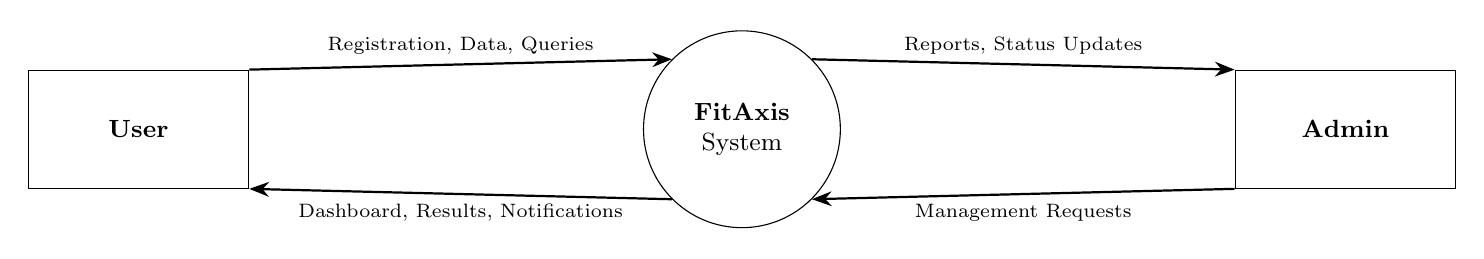
\begin{tikzpicture}

    \node[external, minimum width=2.8cm, minimum height=1.5cm] (user)
        {\textbf{User}};

    \node[process, minimum size=2.5cm, right=5cm of user] (fitaxis)
        {\textbf{FitAxis}\\System};

    \node[external, minimum width=2.8cm, minimum height=1.5cm, right=5cm of fitaxis] (admin)
        {\textbf{Admin}};

    % User -> System
    \draw[dataflow] (user.north east)
        -- node[above, font=\scriptsize] {Registration, Data, Queries}
        (fitaxis.north west);

    % System -> User
    \draw[dataflow] (fitaxis.south west)
        -- node[below, font=\scriptsize] {Dashboard, Results, Notifications}
        (user.south east);

    % System -> Admin
    \draw[dataflow] (fitaxis.north east)
        -- node[above, font=\scriptsize] {Reports, Status Updates}
        (admin.north west);

    % Admin -> System
    \draw[dataflow] (admin.south west)
        -- node[below, font=\scriptsize] {Management Requests}
        (fitaxis.south east);

\end{tikzpicture}
\caption{Data Flow Diagram: Level 0 (Context Diagram)}
\end{figure}

\vspace{1cm}

% =====================================================================
% 5. DFD LEVEL 1
% =====================================================================
\textbf{DFD Level-1:} Decomposition of the FitAxis system into sub-processes.

\begin{figure}[H]
\centering
\resizebox{\textwidth}{!}{%
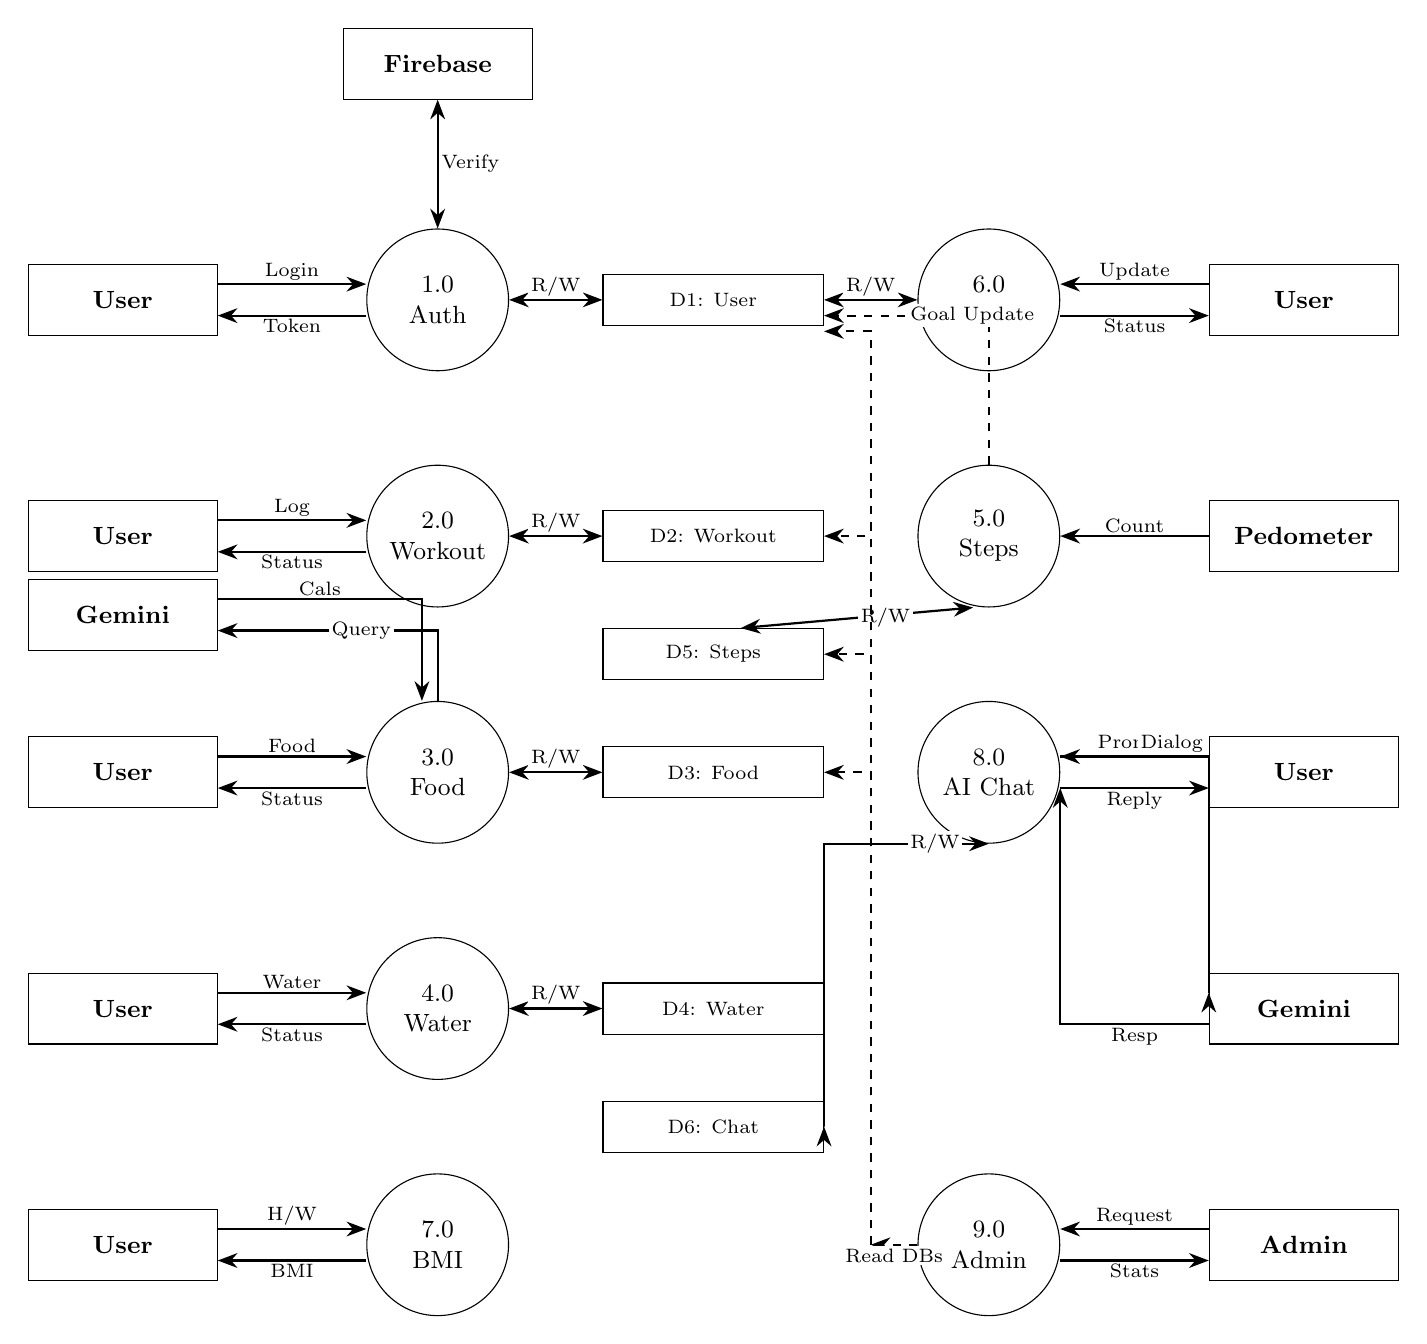
\begin{tikzpicture}

    % ── Replicated External Entities to avoid crossing paths ───────
    \node[external] (u1) at (-7.5, 8) {\textbf{User}};
    \node[external] (u2) at (-7.5, 5) {\textbf{User}};
    \node[external] (u3) at (-7.5, 2) {\textbf{User}};
    \node[external] (u4) at (-7.5, -1) {\textbf{User}};
    \node[external] (u7) at (-7.5, -4) {\textbf{User}};

    \node[external] (u6) at ( 7.5, 8) {\textbf{User}};
    \node[external] (u8) at ( 7.5, 2) {\textbf{User}};
    \node[external] (admin) at (7.5, -4) {\textbf{Admin}};
    
    \node[external] (fbauth)    at (-3.5, 11) {\textbf{Firebase}};
    \node[external] (gemini3)   at (-7.5, 4) {\textbf{Gemini}};
    \node[external] (pedometer) at ( 7.5, 5) {\textbf{Pedometer}};
    \node[external] (gemini8)   at ( 7.5, -1) {\textbf{Gemini}};

    % ── Processes ──────────────────────────────────────────────────
    \node[process] (p1) at (-3.5, 8) {1.0\\Auth};
    \node[process] (p2) at (-3.5, 5) {2.0\\Workout};
    \node[process] (p3) at (-3.5, 2) {3.0\\Food};
    \node[process] (p4) at (-3.5, -1) {4.0\\Water};
    \node[process] (p7) at (-3.5, -4) {7.0\\BMI};

    \node[process] (p6) at ( 3.5, 8) {6.0\\Profile};
    \node[process] (p5) at ( 3.5, 5) {5.0\\Steps};
    \node[process] (p8) at ( 3.5, 2) {8.0\\AI Chat};
    \node[process] (p9) at ( 3.5, -4) {9.0\\Admin};

    % ── Data Stores ────────────────────────────────────────────────
    \node[datastore] (d1) at (0,  8) {D1: User};
    \node[datastore] (d2) at (0,  5) {D2: Workout};
    \node[datastore] (d5) at (0,  3.5) {D5: Steps};
    \node[datastore] (d3) at (0,  2) {D3: Food};
    \node[datastore] (d4) at (0, -1) {D4: Water};
    \node[datastore] (d6) at (0, -2.5) {D6: Chat};

    % ── Flows ──────────────────────────────────────────────────────

    % 1. Auth
    \draw[dataflow] ([yshift=2mm]u1.east) -- node[lbl, above] {Login} ([yshift=2mm]p1.west);
    \draw[dataflow] ([yshift=-2mm]p1.west) -- node[lbl, below] {Token} ([yshift=-2mm]u1.east);
    \draw[biflow]   (p1.east) -- node[lbl, above] {R/W} (d1.west);
    \draw[biflow]   (p1.north) -- node[lbl, right] {Verify} (fbauth.south);

    % 2. Workout
    \draw[dataflow] ([yshift=2mm]u2.east) -- node[lbl, above] {Log} ([yshift=2mm]p2.west);
    \draw[dataflow] ([yshift=-2mm]p2.west) -- node[lbl, below] {Status} ([yshift=-2mm]u2.east);
    \draw[biflow]   (p2.east) -- node[lbl, above] {R/W} (d2.west);

    % 3. Food & Gemini
    \draw[dataflow] ([yshift=2mm]u3.east) -- node[lbl, above] {Food} ([yshift=2mm]p3.west);
    \draw[dataflow] ([yshift=-2mm]p3.west) -- node[lbl, below] {Status} ([yshift=-2mm]u3.east);
    \draw[biflow]   (p3.east) -- node[lbl, above] {R/W} (d3.west);
    \draw[dataflow] (p3.north) |- node[lbl, right, near end] {Query} ([yshift=-2mm]gemini3.east);
    \draw[dataflow] ([yshift=2mm]gemini3.east) -| node[lbl, above, near start] {Cals} ([xshift=-2mm]p3.north);

    % 4. Water
    \draw[dataflow] ([yshift=2mm]u4.east) -- node[lbl, above] {Water} ([yshift=2mm]p4.west);
    \draw[dataflow] ([yshift=-2mm]p4.west) -- node[lbl, below] {Status} ([yshift=-2mm]u4.east);
    \draw[biflow]   (p4.east) -- node[lbl, above] {R/W} (d4.west);

    % 7. BMI
    \draw[dataflow] ([yshift=2mm]u7.east) -- node[lbl, above] {H/W} ([yshift=2mm]p7.west);
    \draw[dataflow] ([yshift=-2mm]p7.west) -- node[lbl, below] {BMI} ([yshift=-2mm]u7.east);

    % 6. Profile
    \draw[dataflow] ([yshift=2mm]u6.west) -- node[lbl, above] {Update} ([yshift=2mm]p6.east);
    \draw[dataflow] ([yshift=-2mm]p6.east) -- node[lbl, below] {Status} ([yshift=-2mm]u6.west);
    \draw[biflow]   (p6.west) -- node[lbl, above] {R/W} (d1.east);

    % 5. Steps
    \draw[dataflow] (pedometer.west) -- node[lbl, above] {Count} (p5.east);
    \draw[biflow]   ([xshift=-2mm]p5.south) -- node[lbl, right] {R/W} ([xshift=3.5mm]d5.north);
    \draw[dataflow, dashed] (p5.north) |- node[lbl, near end, right] {Goal Update} ([yshift=-2mm]d1.east);

    % 8. AI Chat
    \draw[dataflow] ([yshift=2mm]u8.west) -- node[lbl, above] {Prompt} ([yshift=2mm]p8.east);
    \draw[dataflow] ([yshift=-2mm]p8.east) -- node[lbl, below] {Reply} ([yshift=-2mm]u8.west);
    \draw[biflow]   (p8.south) -- node[lbl, right] {R/W} (d6.east |- p8.south) |- (d6.east);
    \draw[dataflow] ([yshift=2mm]p8.east) -- node[lbl, above, near end] {Dialog} ([yshift=2mm]gemini8.west |- p8.east) |- ([yshift=2mm]gemini8.west);
    \draw[dataflow] ([yshift=-2mm]gemini8.west) -| node[lbl, below, near start] {Resp} ([yshift=-2mm]p8.east |- gemini8.west) -- ([yshift=-2mm]p8.east);

    % 9. Admin
    \draw[dataflow] ([yshift=2mm]admin.west) -- node[lbl, above] {Request} ([yshift=2mm]p9.east);
    \draw[dataflow] ([yshift=-2mm]p9.east) -- node[lbl, below] {Stats} ([yshift=-2mm]admin.west);
    
    % Admin DB Read Bus
    \coordinate (bus) at (2, -4);
    \draw[dataflow, dashed] (p9.west) -- node[lbl, below] {Read DBs} (bus);
    \draw[dataflow, dashed] (bus) |- (d5.east);
    \draw[dataflow, dashed] (bus) |- (d3.east);
    \draw[dataflow, dashed] (bus) |- (d2.east);
    \draw[dataflow, dashed] (bus) |- ([yshift=-4mm]d1.east);

\end{tikzpicture}
}%
\caption{Data Flow Diagram: Level 1}
\end{figure}

\end{document}
